%\chapter{Cap\'{\i}tulo 1}
%Los cap\'{\i}tulos son las principales divisiones del documento. En estos, se desarrolla el tema del documento. Cada cap\'{\i}tulo debe corresponder a uno de los temas o aspectos tratados en el documento y por tanto debe llevar un t\'{\i}tulo que indique el contenido del cap\'{\i}tulo.\\
%
%Los t\'{\i}tulos de los cap\'{\i}tulos deben ser concertados entre el alumno y el director de la tesis  o trabajo de investigaci\'{o}n, teniendo en cuenta los lineamientos que cada unidad acad\'{e}mica brinda. As\'{\i} por ejemplo, en algunas facultades se especifica que cada cap\'{\i}tulo debe corresponder a un art\'{\i}culo cient\'{\i}fico, de tal manera que se pueda publicar posteriormente en una revista.\\
%
%\section{Subt\'{\i}tulos nivel 2}
%Toda divisi\'{o}n o cap\'{\i}tulo, a su vez, puede subdividirse en otros niveles y s\'{o}lo se enumera hasta el tercer nivel. Los t\'{\i}tulos de segundo nivel se escriben con min\'{u}scula al margen izquierdo y sin punto final, est\'{a}n separados del texto o contenido por un interlineado posterior de 10 puntos y anterior de 20 puntos (tal y como se presenta en la plantilla).\\
%
%\subsection{Subt\'{\i}tulos nivel 3}
%De la cuarta subdivisi\'{o}n en adelante, cada nueva divisi\'{o}n o \'{\i}tem puede ser se\~{n}alada con vi\~{n}etas, conservando el mismo estilo de \'{e}sta, a lo largo de todo el documento.\\
%
%Las subdivisiones, las vi\~{n}etas y sus textos acompa\~{n}antes deben presentarse sin sangr\'{\i}a y justificados.\\
%
%\begin{itemize}
%\item En caso que sea necesario utilizar vi\~{n}etas, use este formato (vi\~{n}etas cuadradas).
%\end{itemize}

\chapter{Marco teórico}
%
%\section{Black Oil Model}

\section{El medio poroso}

Para entender la física detrás de la simulación de yacimientos de petróleo es necesario revisar el concepto de medio poroso. Un medio poroso puede entenderse como un dominio espacial ocupado parcialmente por un sólido y con una porción ocupada por fluidos a la que se le llama espacio vacío o poroso. Un yacimiento es un medio poroso que ocurre naturalmente, una formación geológica del subsuelo, que, a nivel microscópico, está compuesta por una red de poros que pueden estar interconectados y que almacenan fluidos \citep{Bear2018}.\\

La definición de medio poroso se extiende de la definición de un medio continuo. Un medio continuo, es tal que no pierde sus propiedades al ser dividido infinitamente, es decir, sus propiedades son continuas en todo punto. Sin embargo esta definición, depende del nivel de observación. A nivel microscópico, si se toman medidas de espacio poroso en diferentes puntos, es posible encontrar zonas vacías y otras ocupadas por la roca. Por otro lado, al incrementar el tamaño de la muestra para la medida, es posible notar que las medidas toman valores menos oscilatorios. El mínimo tamaño de muestra al que el espacio poroso empieza a tomar un valor constante se le llama volumen de elemento representativo (REV) \citep{Bear2018}. El espacio poroso medido en un REV, es lo que se denota porosidad ($\phi$), que corresponde a la capacidad de almacenamiento de fluidos a nivel macroscópico.(Acá sería supremamente chimba mostrarlo con un gráfico).\\

%Adicionalmente, existen gargantas de poro que conectan los poros de la roca, estas gargantas de poro indican la capacidad de la roca de permitir el transporte de los fluidos que puedan existir. La propiedad macroscópica que describe de la capacidad de transportar fluido es la permeabilidad absoluta. La permeabilidad absoluta es una propiedad direccional, es decir que puede variar según la dirección en la que se mida, si la permeabilidad varía su dirección en función del espacio, se dice que el medio es anisotrópico.

\section{Transporte de fluidos en medios porosos}

Los fluidos almacenados en el yacimiento en general se encuentran en un estado estable, el cuál se ve afectado por la aplicación de diferentes campos actuando sobre el dominio físico (el medio poroso). Así, los fluidos pueden transportarse debido a efectos gravitacionales, cambios de presión, saturación, entre otros.\\ %En esta tesis de maestría se estudia el flujo o transporte dominado por la advección, es decir, el flujo que se da principalmente por gradientes de presión.

El flujo macroscópico de los fluidos se rige por la ley de conservación de momentum en medios porosos o ley de Darcy que se enuncia en la ecuación \ref{ec:DarcyMonofasico}. Esta ley establece que la velocidad Darcy ($\vec{u}$) de un fluido es proporcional a los gradientes de presión y gravitacionales ($\nabla{\Phi}$ con $\Phi = p - \rho g z$) de un fluido, e inversamente proporcional a su viscosidad ($\mu$). Además, depende de la conductividad del medio poroso, a la cuál, se le denomina permeabilidad absoluta ($\mathbb{K}$).
\begin{align}
	\label{ec:DarcyMonofasico} & \vec{u}=\frac{\mathbb{K}}{\mu } \left(\nabla{\Phi}\right)	
\end{align}

%con $\nabla{\Phi_{f}} = \nabla{p} - \rho g \nabla{z}$ 

donde $\mathbb{K}(\vec{x},t)$ es una propiedad direccional con $\vec{x}=(x,y,z)$:
 
\begin{align}
	\mathbb{K} = \left(\begin{array}{ccc}k_{xx}& & \\
	& k_{yy} & \\
	& & k_{zz}
	\end{array}\right)
\end{align}

Lo anteriormente mencionado, aplica para un solo fluido. En el caso de múltiples fluidos ocupando el espacio poroso se usa la ecuación \ref{ec:DarcyMultifasico}. En ésta, se introduce un término de permeabilidad relativa ($kr_{f}(S_{f})$), que depende de la proporción del volumen poroso ocupado por un fluido, el cuál se denomina saturación ($S_{f}$).

\begin{align}
\label{ec:DarcyMultifasico} & \vec{u_{f}}=\frac{\mathbb{K}kr_{f}}{\mu_{f} } \nabla{\Phi_{f}}
\end{align}

\section{Simulación de Yacimientos de Hidrocarburos}
El dominio de la simulación de yacimientos de hidrocarburos se enmarca dentro del contexto del desarrollo de software científico porque apoya procesos industriales y de investigación de nuevas tecnologías. los cuales requieren la implementación de modelos matemáticos complejos que representan múltiples fenómenos físicos y químicos entre los fluidos.\\

La simulación de yacimientos de hidrocarburos se rige por las leyes de conservación de la masa y del momentum. Estas leyes describen la acumulación, transporte, y fuentes y sumideros de los fluidos como un sistema de ecuaciones diferenciales parciales acopladas para un dominio físico. Solucionar estos sistemas analíticamente, cuando es viable hacerlo, requiere imponer condiciones que se alejan de los problemas reales \citep{ertekin2001basic}. Por lo tanto, es necesario una solución numérica o simulación. Un modelo de simulación ampliamente utilizado en la industria es el \textit{Black Oil Model}.%, este hace una simplificación de la composición de los hidrocarburos existentes. Solucionar tales ecuaciones requiere discretizar el tiempo y el dominio físico; usar métodos de solución de sistemas no lineales, y métodos de solución de sistemas lineales así como el precondicionamiento de los mismos. \\ %Estas elecciones tienen un impacto en las capacidades de solución de ecuaciones que surgen de los diferentes problemas físicos.\\
%Más aún, los resultados de la simulación deben ser contrastados con datos experimentales para verificar su concordancia con el fenómeno físico que modelan.\\


\subsection{Modelo Black Oil Extendido}

El \textit{Black Oil Model} (BOM) es un modelo de conservación de volumen a condiciones estándar. Este considera la existencia de tres fluidos en el medio poroso: aceite, gas y agua. El BOM, asume que el aceite o petróleo, está a condiciones de barril estándar, es decir, a presión y temperatura atmosférica. Además, asume que no existen variaciones considerables en la composición del aceite y del gas \citep{jamal2006petroleum, chen2007reservoir, ertekin2001basic}. Éste modelo considera que puede haber una transferencia de masa en equilibrio desde aceite al gas, lo que se denomina ``Gas disuelto''. Adicionalmente, en el modelo \textit{Black Oil} extendido, se considera una transferencia de masa desde el gas al aceite, lo que se denomina ``aceite volatilizado''. Las ecuaciones de conservación de volumen del BOM se presentan en \ref{ec:aceite}, \ref{ec:gas}, \ref{ec:agua}.

\begin{align}
\label{ec:aceite}
\text{aceite: }&\frac{\partial}{\partial t} \left[ \phi \left( \frac{S_{o}}{B_{o}} + \frac{R_{v} S_{g}}{B_{g}} \right) \right]
- \nabla \cdot \left( \frac{1}{B_{o}} \vec{u_{o}} + \frac{R_{v}}{B_{g}} \vec{u_{g}} \right) + \tilde{q}_{o}=0  \\
\label{ec:gas}
\text{gas: }&\frac{\partial}{\partial t} \left[ \phi \left( \frac{S_{g}}{B_{g}} + \frac{R_{s} S_{o}}{B_{o}} \right) \right]
- \nabla \cdot \left( \frac{1}{B_{g}} \vec{u_{g}} + \frac{R_{s}}{B_{o}} \vec{u_{o}} \right) + \tilde{q}_{g} = 0 \\
\label{ec:agua}
\text{agua: }&\frac{\partial}{\partial t} \left[\phi \left( \frac{S_{w}}{B_{w}} \right) \right] - \nabla \cdot \left( \frac{1}{B_{w}} \vec{u_{w}} \right) + \tilde{q}_{w} = 0 
\end{align}
donde $\vec{u_{f}}$ corresponde a la velocidad Darcy, y, $\tilde{q}_{f}$ a los aportes de fuentes y sumideros, que posteriormente serán modelados como pozos, para el fluido $f = \left\lbrace o:\text{ aceite}, g:\text{ gas}, w:\text{ agua} \right\rbrace $.\\

En el BOM se establece, también, que los fluidos tienen una compresibilidad, es decir que cambian su volumen según la presión a la que estén sometidos. La propiedad asociada a ese cambio de volumen es el factor volumétrico ($B_{f}$).
%\begin{equation*}
%\vec{u_{f}}=\frac{\mathbb{K}kr_{f}}{\mu_{f} } \nabla{\Phi_{f}}
%\end{equation*}

%con $\nabla{\Phi_{f}} = \nabla{p} - \rho g \nabla{z}$.

\subsection{Problema de Valores Iniciales}

En el desarrollo de esta tesis, se consideran yacimientos con condiciones de borde cerradas o Neumann cero para todas las fronteras. Es decir, no existen acuíferos aportando presión o caudal en yacimiento. Las diferencias de presión se generan por la presencia de pozos productores e inyectores.\\

(Poner un dibujito de un yacimiento con pozos.)

Además para un tiempo $t=0$ se tiene que:
\begin{align}
	P_{f}(\vec{x},0) = P^{0}_{f}(\vec{x}) \qquad \forall f \in \left\lbrace o,g,w\right\rbrace\\
	S_{f}(\vec{x},0) = S^{0}_{f}(\vec{x}) \qquad \forall f \in \left\lbrace o,g,w\right\rbrace
\end{align}
%
Es decir, existe funciones en el espacio que describen las condiciones iniciales de presión $P^{0}_{f}(\vec{x})$ y saturación $S^{0}_{f}(\vec{x})$ para los fluidos $f$ del yacimiento.

\subsection{Discretización}

Se elije el método de los volúmenes finitos para las discretización espacial de las ecuaciones \ref{ec:aceite}, \ref{ec:gas} y \ref{ec:agua} y un esquema implícito para la discretización del tiempo, es decir, elección del tiempo al $n+1$ (futuro). El proceso de discretización se muestra en el anexo \ref{AnexoA}. Para una celda con índice $i$ con superficie $S$ como un conjunto de caras $c$, la discretización de las ecuaciones es la siguiente:
%Algebraic Equations
\begin{align}
\label{ec:aceiteDiscretizacion}&\underbrace{\frac{|\Omega_{i}|}{\Delta t}\left[ \phi^{t}_{i} \left( \frac{S_{o,i}^{t}}{B_{o,i}^{t}} + \frac{Rv_{i}^{t}S_{g,i}^{t}}{B_{g,i}^{t}}\right)\right]^{n+1}_{n}}_{\text{Acumulación - Aceite}} + 
\underbrace{\sum_{c \in S}\left[ T^{n+1}_{o,c} \nabla{\Phi_{o,c}^{n+1}} + Rv_{c}T^{n+1}_{g,c} \nabla{\Phi_{g,c}^{n+1}} \right] }_{\text{Flujo - Aceite}}+ \dot{Q}_{o,i}^{n+1} = 0 \\
\label{ec:gasDiscretizacion}&\underbrace{\frac{|\Omega_{i}|}{\Delta t}\left[ \phi^{t}_{i} \left( \frac{S_{g,i}^{t}}{B_{g,i}^{t}} + \frac{Rs_{i}^{t}S_{o,i}^{t}}{B_{o,i}^{t}}\right)\right]^{n+1}_{n}}_{\text{Acumulación - Gas}} + 
\underbrace{\sum_{c \in S}\left[ T^{n+1}_{g,c}\nabla{\Phi_{g,c}^{n+1} + Rs_{c}T^{n+1}_{o,c} \nabla{\Phi_{o,c}^{n+1}}} \right] }_{\text{Flujo - Gas}}+ Q_{g,i}^{n+1} = 0 \\
\label{ec:aguaDiscretizacion}&\underbrace{\frac{|\Omega_{i}|}{\Delta t}\left[ \phi^{t}_{i} \left( \frac{S_{w,i}^{t}}{B_{w,i}^{t}}\right)\right]^{n+1}_{n}}_{\text{Acumulación - Agua}}
+ 
\underbrace{\sum_{c \in S}\left[ T^{n+1}_{w,c}\nabla{\Phi_{w,c}^{n+1}} \right]}_{\text{Flujo - Agua}} + Q_{w,i}^{n+1} = 0 
\end{align}

dónde:

\begin{align*}
	&\left[ \phi^{t}_{i} \left( \frac{S_{o,i}^{t}}{B_{o,i}^{t}} + \frac{Rv_{i}^{t}S_{g,i}^{t}}{B_{g,i}^{t}}\right)\right]^{n+1}_{n} = 
	\phi^{n+1}_{i} \left( \frac{S_{o,i}^{n+1}}{B_{o,i}^{n+1}} + \frac{Rv_{i}^{n+1}S_{g,i}^{n+1}}{B_{g,i}^{n+1}}\right) - \phi^{n}_{i} \left( \frac{S_{o,i}^{n}}{B_{o,i}^{n}} + \frac{Rv_{i}^{n}S_{g,i}^{n}}{B_{g,i}^{n}}\right),\\
	&\left[ \phi^{t}_{i} \left( \frac{S_{g,i}^{t}}{B_{g,i}^{t}} + \frac{Rs_{i}^{t}S_{o,i}^{t}}{B_{o,i}^{t}}\right)\right]^{n+1}_{n} = 
	\phi^{n+1}_{i} \left( \frac{S_{g,i}^{n+1}}{B_{g,i}^{n+1}} + \frac{Rs_{i}^{n+1}S_{o,i}^{n+1}}{B_{o,i}^{n+1}}\right) - \phi^{n}_{i} \left( \frac{S_{g,i}^{n}}{B_{g,i}^{n}} + \frac{Rs_{i}^{n}S_{o,i}^{n}}{B_{o,i}^{n}}\right),\\
	&\left[ \phi^{t}_{i} \left( \frac{S_{w,i}^{t}}{B_{w,i}^{t}}\right)\right]^{n+1}_{n} = 
	\phi^{n+1}_{i} \left( \frac{S_{w,i}^{n+1}}{B_{w,i}^{n+1}}\right) - \phi^{n}_{i} \left( \frac{S_{w,i}^{n}}{B_{w,i}^{n}}\right)
\end{align*}

El término $T_{f,c}$ en la ecuación \ref{ec:Transmissibity} corresponde a la transmisividad en una cara $c$ que conecta una celda $i$ con otra celda $j$.

\begin{align}
	\label{ec:Transmissibity}& T_{f,c} = \left(\frac{1}{(\Delta l_{i}/A_{c}K_{l,i})+(\Delta l_{j}/A_{c}K_{l,j})}\right)\frac{kr_{f}}{\mu_{f}B_{f}}
\end{align}
\subsection{Modelado de Pozos}
%
Al establecer condiciones de frontera cerradas es necesario perforar pozos para generar diferencias de presión que induzcan al transporte de los hidrocarburos presentes en el yacimiento. Los pozos tienen dos tipos, inyector o productor.

\begin{align}
	q^{(v)} = \sum_{m=1}^{M^{(v)}_{w}}\frac{2\pi\rho\sqrt{k_{xx}k_{yy}}h_{z}}{\mu\left(r_{e}/r_{w} +s\right)}\left(p_{bh}^{(v)}-p_{m}-\gamma\left(z_{bh}^{(v)}-z_{m}\right)\right)\delta\left(x-x_{m}^{(v)}\right)
\end{align}
%
\subsection{Método de Newton-Raphson}
%
El sistema de ecuaciones algebraicas formado por \ref{ec:aceiteDiscretizacion}, \ref{ec:gasDiscretizacion} y \ref{ec:aguaDiscretizacion} es no lineal. Por lo tanto, se aplica el método del Newton-Raphson el cuál se usa para encontrar las raíces de una ecuación no lineal aproximándose por su derivada como se ilustra en la imagen \ref{fig:Newton}.
\begin{equation}
A \cdot {\Delta \vec{x}} = \vec{b} \Leftrightarrow J^{k}_{i,j} \cdot {\Delta \vec{x}} = -\vec{R^{k}_{i}}
\end{equation}
\begin{equation}
\Delta \vec{x} = \vec{x}^{k+1} - \vec{x}^{k} = \left(\Delta P_o, \Delta S_g, \Delta S_w \right)^T
\end{equation}
\begin{equation}
-\vec{R^k_i} = \left(\Delta R^k_{P_o,i}, \Delta R^k_{S_g,i}, \Delta R^k_{S_w,i} \right)^T
\end{equation}
\begin{equation}
J^k_{i,j}=\frac{\partial R^k_i}{\partial x^k_j}	
\end{equation}
\begin{equation}
\frac{\partial R^k}{\partial x^k} \approx \frac{R\left(x^k + \xi \right) - R\left(x^k \right)}{\xi}
\end{equation}
%\section{Procesos de Recobro Mejorado}

%\subsection{Modelamiento del Químico}

\section{Esquemas Preconceptuales}

Los Esquemas Preconceptuales (EP) son representaciones intermedias entre el lenguaje natural y un esquema conceptual o un lenguaje formal. Estos esquemas contienen todo el dominio de aplicación de un interesado, y por tanto, sirven para establecer un punto común de entendimiento entre un interesado y un analista de software \citep{zapata2007phd}. Los EP se desarrollan con la idea de mantener la coherencia y consistencia entre el discurso del interesado y el software desarrollado. 

\subsection{Elementos del Esquema Preconceptual}
\cite{zapata2012unc} define los elementos del EP tal como se observa en la figura \ref{fig:InitialPS} para la representación del dominio del interesado. Estos elementos se dividen en cuatro categorías: nodos, relaciones, enlaces, y agrupadores.\\

\begin{figure}[h]
	\centering%
	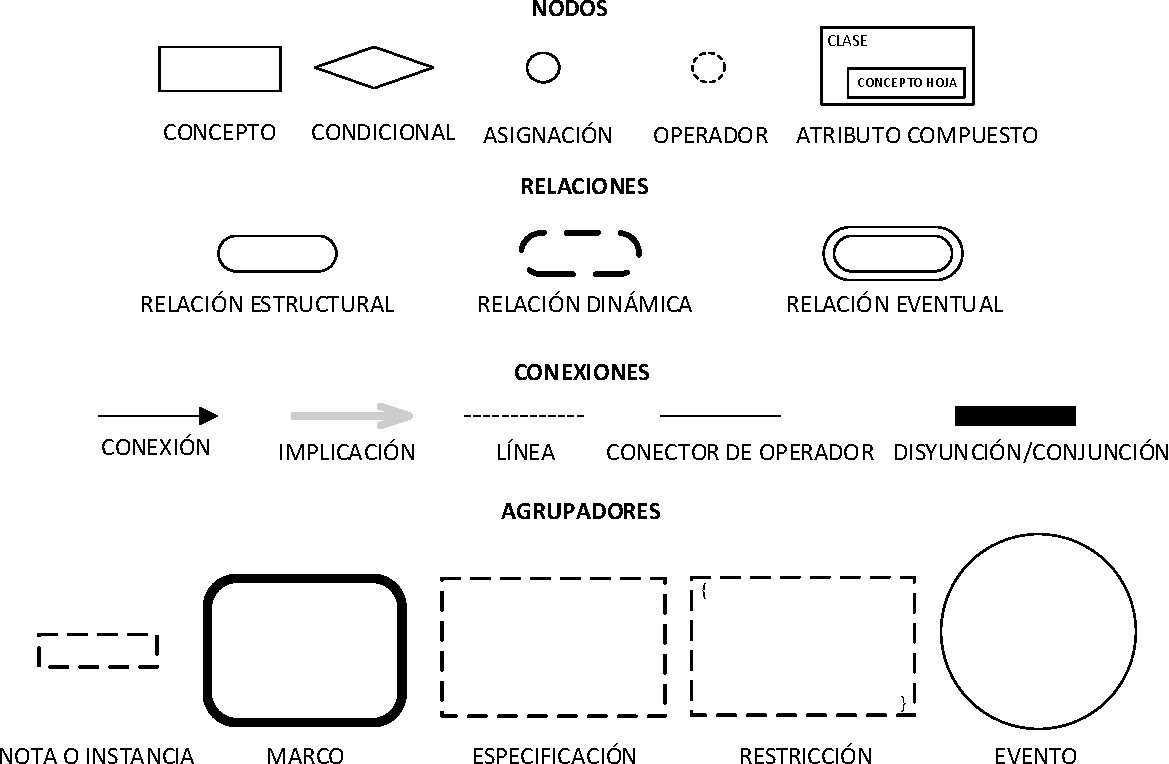
\includegraphics[scale=0.51]{Fig/ElementosDelEP.pdf}%
	\caption[Elementos del EP.]{Elementos del EP. Tomado de \citep{zapata2012unc}.} \label{fig:InitialPS}
\end{figure}

\subsubsection{Nodos}
\begin{itemize}
	\item \textbf{Concepto}:
	Los conceptos son sustantivos o sintagmas nominales que representan un actor u objeto dentro del dominio del interesado, se subclasifican en conceptos clase y conceptos hoja, según su jerarquía \citep{zapata2007phd,zapata2012unc}. %En la figura \ref{fig:PS_Concept} se muestra la representación. Un ejemplo de su uso se presenta en la figura \ref{fig:ej_concept}.
	
	\item \textbf{Condicional}: Los condicionales establecen cuando ejecutar una relación dinámica o una especificación a partir de una expresión lógica formada por conceptos o variables, operadores, y valores o parámetros \citep{zapata2007phd,zapata2012unc}. %como se muestra en la figura \ref{fig:}
	
	\item \textbf{Operador}: Los operadores son símbolos lógicos o matemáticos que sirven para formar expresiones a evaluar \citep{zapata2012unc}.
	
	\item \textbf{Asignación}: Sirve para asignar el valor que resulta de una expresión matemática o lógica \citep{zapata2012unc}.
	
	\item \textbf{Atributo Compuesto}: Sirve para representar el acceso a un concepto hoja o atributo desde su concepto clase \citep{zapata2007phd}.
\end{itemize}

\subsubsection{Relaciones}
\begin{itemize}
	\item \textbf{Relación Estructural}: Relaciones permanentes entre dos conceptos, se asocian a los verbos ``ser'' o ``tener'' y establecen generalización o agregación, respectivamente \citep{zapata2007phd,zapata2012unc}.
	\item \textbf{Relación Dinámica}: Se asocian a verbos que denotan acción u operaciones que modifican el dominio de estudio, establecen relaciones transitorias entre el concepto ejecutor de la acción con el concepto objeto de dicha acción \citep{zapata2007phd,zapata2012unc}.
	\item \textbf{Relación Eventual}: Se relaciona con un verbo que denota ocurrencia \citep{zapata2012unc,norena2018Ling}.
\end{itemize}

\subsubsection{Enlaces}
\begin{itemize}
	\item \textbf{Conexión}: Es una flecha unidireccional que sirve para conectar conceptos con relaciones dinámicas o estructurales \citep{zapata2007phd,zapata2012unc}.
	\item \textbf{Implicación}: Es una línea continua y dirigida que sirve para indicar una relación causa-efecto u orden entre relaciones dinámicas, condicionales o eventos. \citep{zapata2007phd,zapata2012unc}. 
	\item \textbf{Línea}: Sirve para conectar un concepto a una nota o instancia \citep{zapata2007phd,zapata2012unc}.
	\item \textbf{Conector de Operador}: Sirve para conectar un valor, concepto, atributo compuesto u otros operadores, a un operador \citep{zapata2012unc}. 
	\item \textbf{Conjunción/Disyunción}: Sirve para agrupar o bifurcar implicaciones, estableciendo una causalidad conjunta o múltiples efectos \citep{zapata2007phd,zapata2012unc}. 
\end{itemize}

\subsubsection{Agrupadores}
\begin{itemize}
	\item \textbf{Nota o Instancia}: Sirve para limitar los valores para un concepto a un conjunto predefinido \citep{zapata2007phd,zapata2012unc}.
	\item \textbf{Especificación}: Sirve para agrupar un conjunto de operaciones que describen una relación dinámica o eventual \citep{zapata2012unc}.
	\item \textbf{Marco}: Sirve para asociar múltiples relaciones dinámicas a una responsabilidad o para agrupar conceptos \citep{zapata2012unc}.
	\item \textbf{Restricción}: Sirve para establecer una condición sobre una especificación de operaciones \citep{zapata2012unc}. Adicionalmente, se usa para establecer ciclos sobre conceptos o condiciones \citep{JChaverra}.
	\item \textbf{Evento}: Es una ocurrencia que habilita cambios de estado en los procesos  \citep{zapata2013Eventos}.
\end{itemize}

\subsection{Esquemas Preconceptuales en el contexto del software científico}

\cite{JCalle, norena2018det} descubren la capacidad del EP para representar aplicaciones en el contexto del software científico. Para ello, definen elementos adicionales que permiten modelar dominios de mayor complejidad. En esta tesis de maestría se usan las condiciones iniciales, conceptos tipo arreglo, parámetros, variables, vectores, operadores predefinidos, operador ``push'', operador ``type'',  y funciones definidas por el analista. En la figura \ref{fig:NewElements} se presenta la representación de los elementos previamente mencionados. A continuación, se explican los elementos adicionales que se usan en el desarrollo de esta tesis.

\begin{figure}[h]
	\centering%
	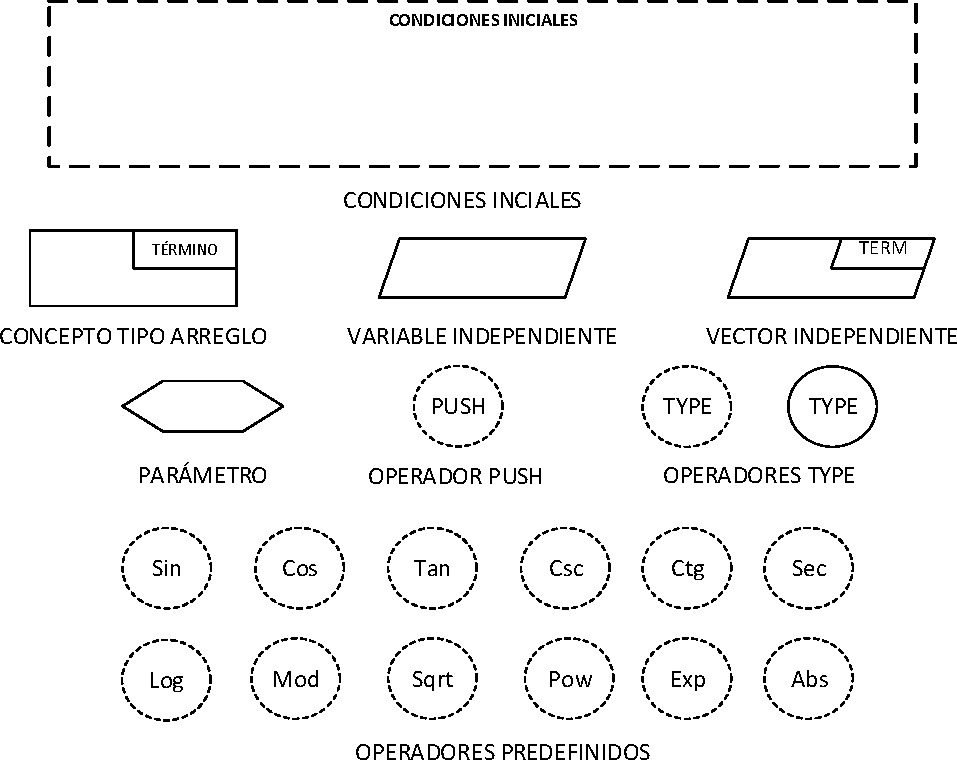
\includegraphics[width=0.9\linewidth]{Fig/NuevosElementosDelEP.pdf}%
	\caption[Elementos para la representación de Software Científico.]{Elementos para la representación de Software Científico. Los autores a partir de \citep{JCalle,norena2018det}.} \label{fig:NewElements}
\end{figure}

\subsubsection{Condiciones Iniciales}
Las condiciones iniciales son una especificación, de variables y parámetros globales, que se conoce desde el inicio de la simulación \citep{norena2018det}. Un ejemplo de uso se presenta en la figura \ref{fig:EjInitialConditions}.

\begin{figure}[h]
	\centering%
	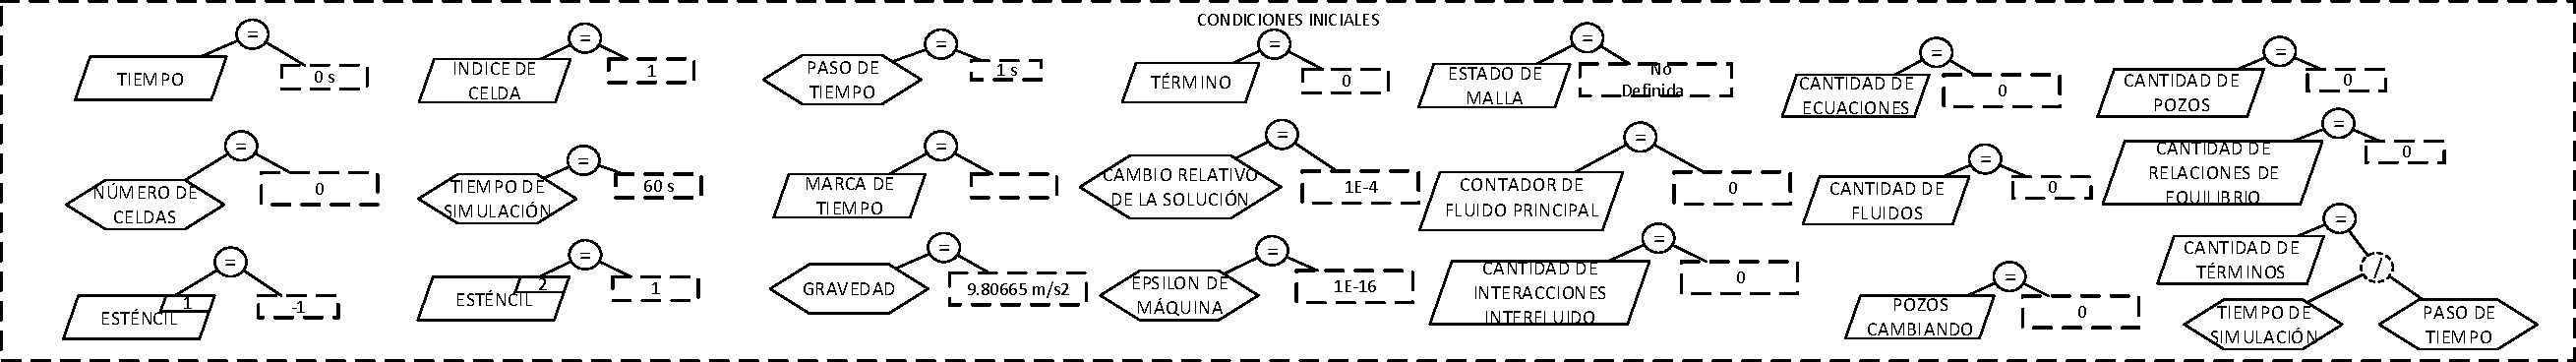
\includegraphics[width=0.9\linewidth]{Fig/EjInitialConditions.pdf}%
	\caption[Condiciones Iniciales.]{Condiciones Iniciales. Los autores.} \label{fig:EjInitialConditions}
\end{figure}

\subsubsection{Concepto tipo arreglo}
Los conceptos tipo arreglo permiten almacenar de manera permanente múltiples valores, y a su vez, iterar sobre ellos \citep{JCalle}. En esta tesis de maestría se usan conceptos tipo arreglos multidimensionales. En la figura \ref{fig:EjArrConcept} se expone un ejemplo de su uso.

\begin{figure}[h]
	\centering%
	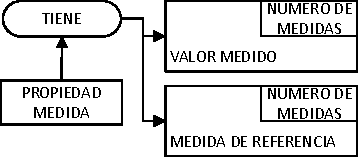
\includegraphics[scale=1]{Fig/EjArrConcepts.pdf}%
	\caption[Conceptos tipo arreglo.]{Conceptos tipo arreglo. Los autores.} \label{fig:EjArrConcept}
\end{figure}

\subsubsection{Parámetro}
Los parámetros se usan para almacenar constantes o definir entradas en la especificación de relaciones dinámicas, especificaciones de tipo marco y, funciones, que reciben múltiples argumentos o parámetros \citep{JCalle, norena2018det}. Se expone un ejemplo de uso en \ref{fig:EjParameter}.\\

\begin{figure}[h]
	\centering%
	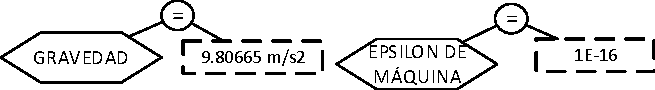
\includegraphics[width=0.5\linewidth]{Fig/EjParametro.pdf}%
	\caption[Ejemplo de parámetros.]{Ejemplo de parámetros. Los autores.} \label{fig:EjParameter}
\end{figure}

\subsubsection{Variable Independiente}
Las variables independientes permiten almacenar valores durante la ejecución de una especificación sin estar acopladas a un concepto. Si se definen en las condiciones iniciales, se pueden usan de manera global durante toda la simulación \citep{norena2018det}. En la figura \ref{fig:EjInitialConditions} se pueden ver ejemplos de variables independientes.\\

\subsubsection{Vector independiente}
Los vectores independientes cumplen la misma tarea y propiedades de las variables independientes pero permiten almacenar más de un valor \citep{norena2018det}. Un ejemplo de vector independiente se presenta en \ref{fig:EjVector}.

\begin{figure}[h]
	\centering%
	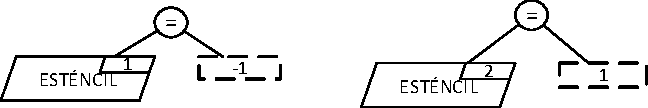
\includegraphics[width=0.5\linewidth]{Fig/EjVectorIndependiente.pdf}%
	\caption[Ejemplo de vector independiente.]{Ejemplo de vector independiente. Los autores.} \label{fig:EjVector}
\end{figure}

\subsubsection{Operadores Predefinidos}
Son funciones algebraicas y trigonométricas predefinidas que se pueden usar como operadores en el EP \citep{JCalle}.

\subsubsection{Operador Push}
El operador Push sirve para insertar, valores, conceptos o parámetros dentro de un concepto tipo arreglo, el elemento que se inserta queda en la última posición del arreglo  \citep{JCalle}.
\subsubsection{Operador Type}
El operador Type tiene dos versiones, una como operador de asignación y otro como operador de información. En el caso de la asignación, sirve para otorgarle el tipo de una subclase a un concepto. Mientras que en el de información, consulta si el tipo del concepto corresponde con el tipo de una subclase definida \citep{JCalle}.
\subsubsection{Funciones definidas por el analista}
Las funciones definidas por el analista son especificaciones reutilizables en el EP a modo de un operador personalizado cuyo nombre define el analista. Éstas funciones llevan en su especificación un concepto ``return'' que corresponde al valor que devuelve la función al ser usada como operador \citep{JCalle}. En la figura \ref{fig:Potencial} se presenta un ejemplo de definición y uso de una función definida por el analista.

\begin{figure}[h]
	\centering%
	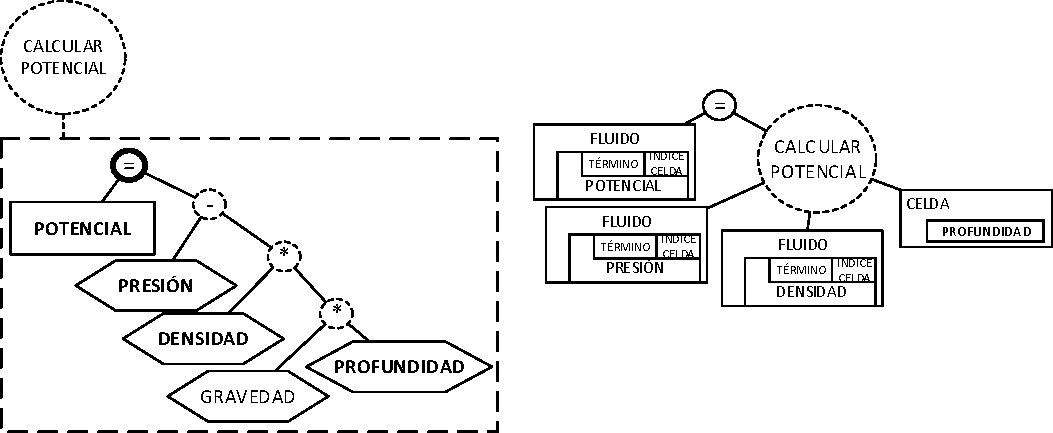
\includegraphics[scale=0.8]{Fig/EjFuncion.pdf}%
	\caption[Ejemplo de función, cálculo del potencial.]{Ejemplo de función, cálculo del potencial. Los autores.} \label{fig:Potencial}
\end{figure}

